\chapter{Resultados y Validación}\label{chapter:resultsValidation}
\label{sec:17}

    El objetivo de esta sección radica en demostrar el uso de este sistema y validarlo. Se usó el modelo SIR, SI para evaluar el modelo, para ello se estimaron 120 días
     de epidemia con diferentes parámetros. Se añadió error a las estimaciones para conseguir intervalos de incertidumbre. \\

        \subsection*{Presentación y análisis de los resultados obtenidos a partir del algoritmo propuesto}  

        Modelo SIR: Divide la población en tres grupos: Susceptibles (S), Infectados (I) y Recuperados (R), los supuestos del modelo SIR son población cerrada, no hay 
        nacimientos, muertes ni migración (\(N = S + I + R = \text{constante}\)). Contactos homogéneos, todos los individuos interactúan entre sí de manera uniforme. 
        Inmunidad permanente, los recuperados no vuelven a ser susceptibles. Tasas constantes, La tasa de transmisión (\(\beta\)) y de recuperación (\(\gamma\)) 
        son constantes. \\
        
        Variables y Parámetros:
        \begin{enumerate}
            
            \item \(S(t)\): Número de susceptibles en el tiempo \(t\).
            \item \(I(t)\): Número de infectados en el tiempo \(t\).
            \item \(R(t)\): Número de recuperados (o removidos) en el tiempo \(t\).
            \item \(N\): Población total (\(N = S + I + R\)).
            \item \(\beta\): Tasa de transmisión (probabilidad de contagio por contacto).
            \item \(\gamma\): Tasa de recuperación (fracción de infectados que se recuperan por unidad de tiempo).
            \item \(R_0\): Número reproductivo básico (\(R_0 = \frac{\beta}{\gamma}\)). \\
        \end{enumerate}

        \textbf{Sistema de ecuaciones diferenciales ordinarias (EDOs):}
        \begin{enumerate}
            
            \item  Tasa de cambio de los susceptibles:
               \[
               \frac{dS}{dt} = -\frac{\beta}{N} S I
               \]
            \item Tasa de cambio de los infectados:
                  \[
                  \frac{dI}{dt} = \frac{\beta}{N} S I - \gamma I
                  \]
            \item Tasa de cambio de los recuperados:
                \[
                \frac{dR}{dt} = \gamma I
                \]
               
        \end{enumerate}

        Las siguientes figuras muestran el intervalo de los valores $S_0,I_0,R_0$ de una epidemia que se propaga por 120 dias. \\

        \begin{center}
            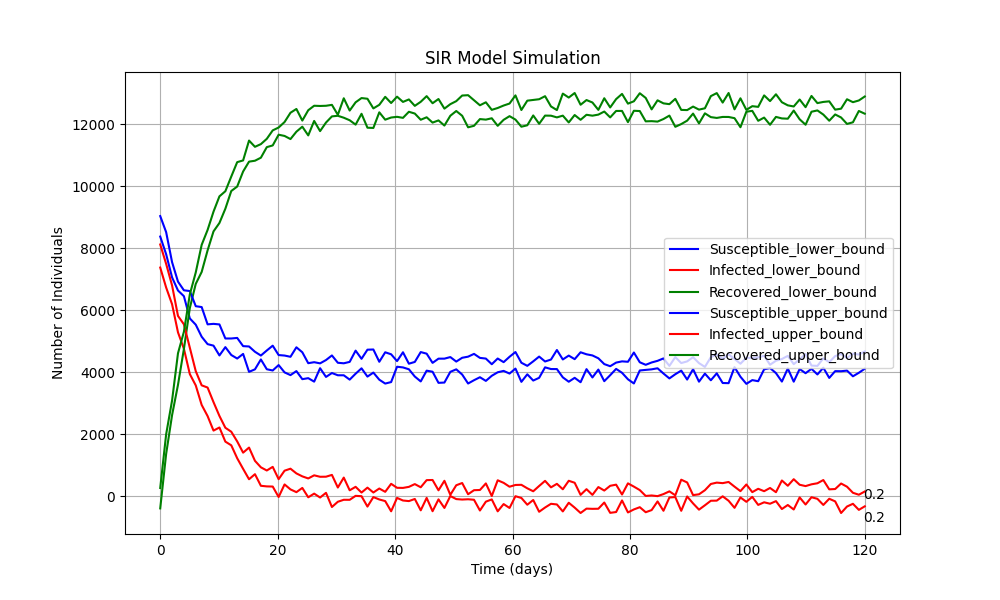
\includegraphics[width=0.6\textwidth]{images/plot0.png}
            \begin{center}
               fig.2 Parámetros  gamma = 0.2, beta = 0.2
            \end{center}
            
            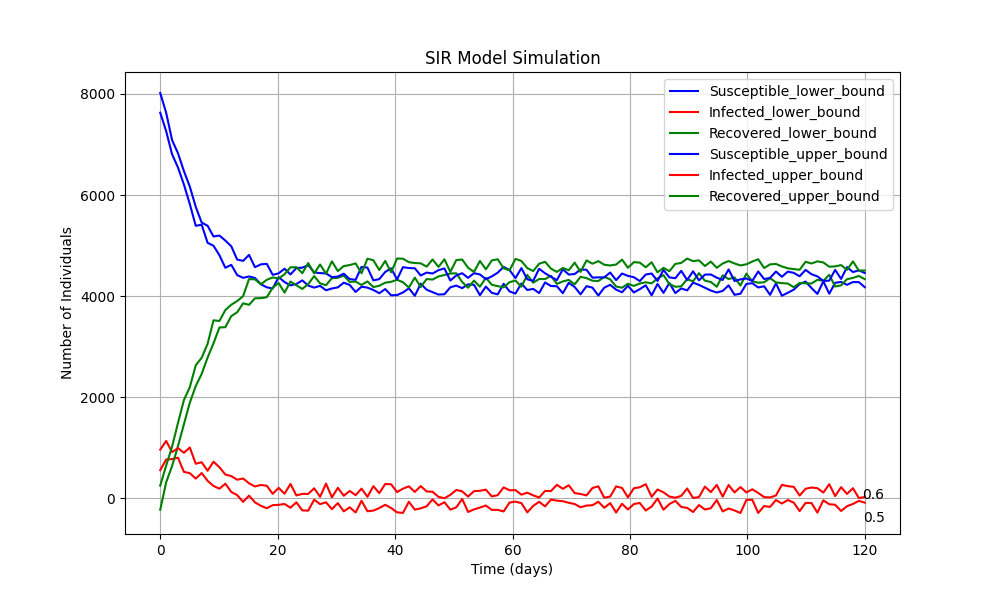
\includegraphics[width=0.6\textwidth]{images/plot1.png}
            \begin{center}
                fig.3 Parámetros  gamma = 0.6, beta = 0.5
            \end{center}
            
            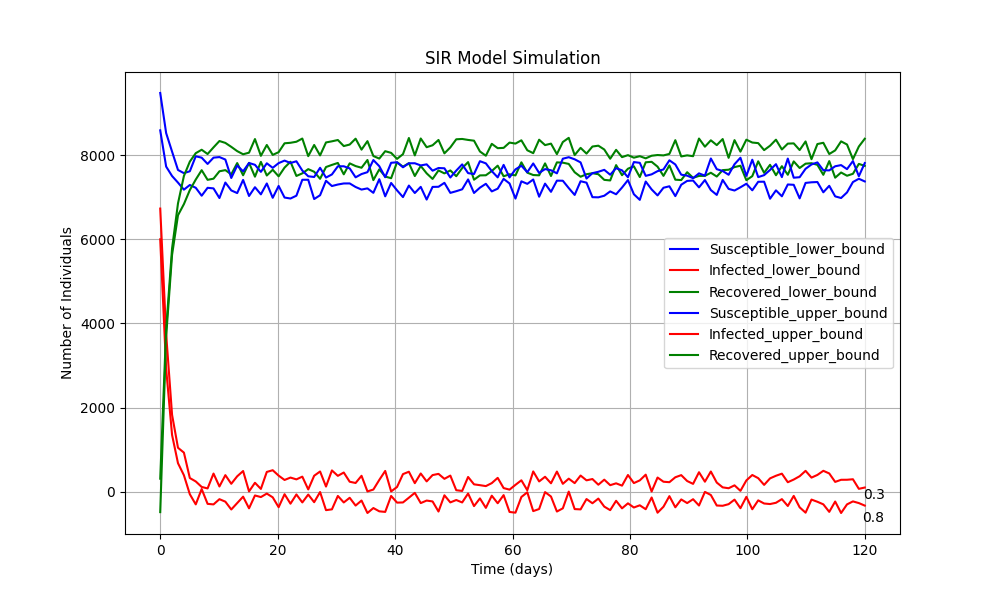
\includegraphics[width=0.6\textwidth]{images/plot2.png}
            \begin{center}
                fig.4 Parámetros  gamma = 0.3, beta = 0.8
            \end{center}
            
            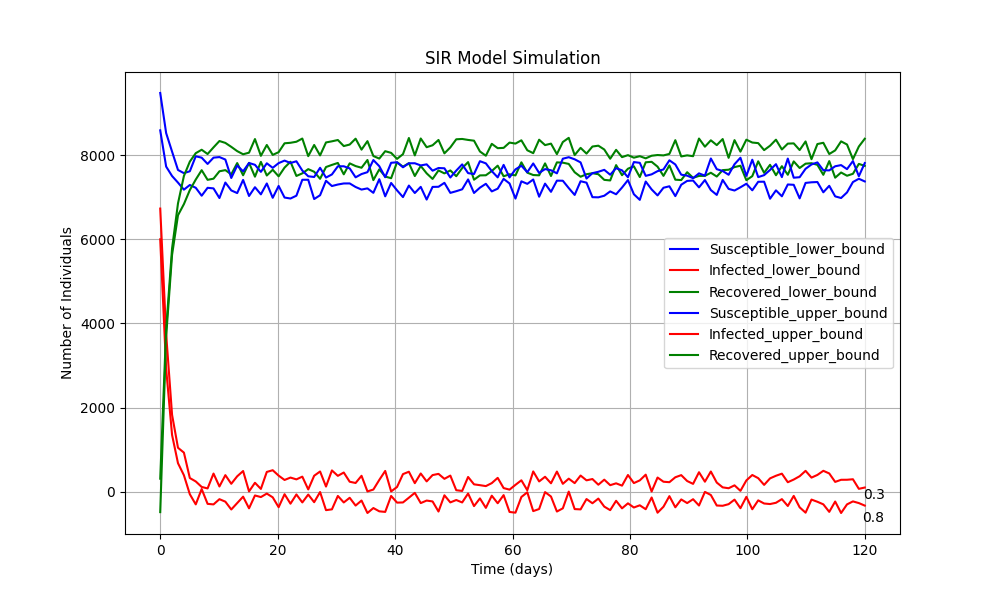
\includegraphics[width=0.6\textwidth]{images/plot2.png}
            \begin{center}
                fig.5 Parámetros  gamma = 0.3, beta = 0.7
            \end{center}
    \end{center}


    Las funciones usadas en los agentes fueron: \\
    \begin{enumerate}
        
        \item  Función identidad
           \( f(x) = x \)  
           \( f^{-1}(y) = y \)
        
           \item  Escalar lineal  
           \( f(x) = 2x \)  
           \( f^{-1}(y) = \frac{y}{2} \)
        
           \item  Trasformación afín
           \( f(x) = 3x + 1 \)  
           \( f^{-1}(y) = \frac{y - 1}{3} \)
        
           \item  Función cúbica
           \( f(x) = x^3 \)  
           \( f^{-1}(y) = y^{1/3} \)
        
           \item  Función exponencial  
           \( f(x) = e^x \)  
           \( f^{-1}(y) = \ln(y) \)
        
           \item  Logaritmo natural
           \( f(x) = \ln(x) \)  
           \( f^{-1}(y) = e^y \)
        
           \item  Función seno
           \( f(x) = \sin(x) \)  
           \( f^{-1}(y) = \arcsin(y) \)
        
           \item  Función tangente  
           \( f(x) = \tan(x) \)  
           \( f^{-1}(y) = \arctan(y) \)
        
           \item  Función recíproco  
           \( f(x) = \frac{1}{x} \) (definida si \( 0 \notin x \))  
           \( f^{-1}(y) = \frac{1}{y} \) (definida si \( 0 \notin y \))  
           
        
           \item  Función coseno
            \( f(x) = \cos(x) \)  
            \( f^{-1}(y) = \text{arccosh}(y) \)  
            
        
            \item  Función sigmoidal
            \( f(x) = \frac{1}{1 + e^{-x}} \)  
            \( f^{-1}(y) = \ln\left(\frac{y}{1 - y}\right) \)
        
            \item  Función seno hiperbólico
            \( f(x) = \sinh(x) \)  
            \( f^{-1}(y) = \text{arcsinh}(y) \)  
            
        
            \item  Función coseno hiperbólico
            \( f(x) = \cosh(x) \)  
            \( f^{-1}(y) = \text{arccosh}(y) \)
        
            \item  Función arco tangente
            \( f(x) = \arctan(x) \)  
            \( f^{-1}(y) = \tan(y) \)
        
            \item  Función Logit
            \( f(x) = \ln\left(\frac{x}{1 - x}\right) \)  
            \( f^{-1}(y) = \frac{1}{1 + e^{-y}} \)
        
            \item  Función cúbica
            \( f(x) = x^{1/3} \)  
            \( f^{-1}(y) = y^3 \)
        
            \item Función componente lineal  
            \( f(x) = 1 - x \)  
            \( f^{-1}(y) = 1 - y \)
        
            \item  Función logaritmo Base-10   
            \( f(x) = \log_{10}(x) \)  
            \( f^{-1}(y) = 10^y \)

    \end{enumerate}


    \textbf{Agente coordinador:} \\

    El agente coordinador usado fue random forest que es una colección de árboles predictores, donde cada árbol depende del valor de un vector aleatorio probado
     independientemente y con la misma distribución para cada uno. Este algoritmo combina las ideas del bagging (bootstrap aggregating) y la selección aleatoria 
     de atributos (random subspace) para construir una colección diversa e independiente de árboles. 
     
    Funcionamiento: Se selecciona un subconjunto aleatorio tanto del conjunto total de datos como del conjunto total de características o atributos disponibles. 
    Esto se hace mediante técnicas como el bootstrapping (muestreo con reemplazo). Para cada muestra seleccionada, se construye un árbol individual usando solo 
    una porción aleatoria del conjunto completo de características disponibles en cada nodo interno. Esto ayuda a reducir el riesgo sobreajuste (overfitting) al 
    aumentar la diversidad entre los diferentes modelos. Cada nuevo dato que se desee predecir pasa por todos los árboles individuales generados durante el 
    entrenamiento. En clasificación, el resultado final es determinado por votación mayoritaria entre todos los resultados obtenidos; mientras que en regresión, 
    se toma el promedio aritmético. \\

    Ventajas: Los Random Forests suelen ofrecer resultados más precisos que otros métodos debido a su capacidad para combinar múltiples predicciones. Al utilizar 
    subconjuntos aleatorios tanto en datos como características, reduce significativamente el riesgo sobreajuste. Pueden manejar variables continuas y categóricas 
    simultáneamente. Comparado con otros métodos avanzados, requiere menos ajustes manuales complejos. \\
    
    Sin embargo, también tiene algunas desventajas como alto costo computacional especialmente con grandes conjuntos y dificultad interpretativa debido a su 
    complejidad interna. \\

    El motivo principal de su selección radica en su uso sencillo y adaptabilidad a la entrada de un vector $k$ de parámetros y $k^2$ salidas, puesto que el problema 
    de encontrar el grafo $G$ se puede pensar como un problema de clasificación en el que se tiene $k^2$ clases. También se comprobó que epíricamente que sus resultados
    eran numéricamente estables, algo que resultó muy importante para este desarrollo. \\


    \textbf{Implementación de intervalos y estabilidad numérica:}

    Si bien los intervalos ofrecen una forma de atacar la incertidumbre en los datos, es un desafío para calcular $f(X)$ siendo $X$ un intervalo en el cual no 
    necesariamente se define la función, es decir, si un gente $A$ recibe una entrada $X$ esta entrada puede no ser reconocible por este, por tanto se requiere 
    implementar herísticas para mantener la estabiliada numérica y la armonía del sistema(que no termine en excepción). Muchas de las técnicas usadas provocaron 
    inestabiliada en la solución calculada por estos agentes y se usaron como dato de entrenamiento para que el agente coordinador determine que los datos $X$ no 
    son reconocibles por el agente $A$. \\

    \textbf{El entrenamiento:}

    El sistema iteró solo una época por los datos de entrenamiento con una constante de hasta 100 iteraciones por cada dato para devolver una salida, se consideraron un total de 150 epidemias. 
    A continuación se muestran gráficas para ilustrar este proceso. El numero total de iteraciones fue de 15000 consiguiendose el siguiente cronograma de salidas.

    \begin{center}
        
        
\includegraphics[width=0.6\textwidth]{images/1.png}

        
\includegraphics[width=0.6\textwidth]{images/2.png}
        
        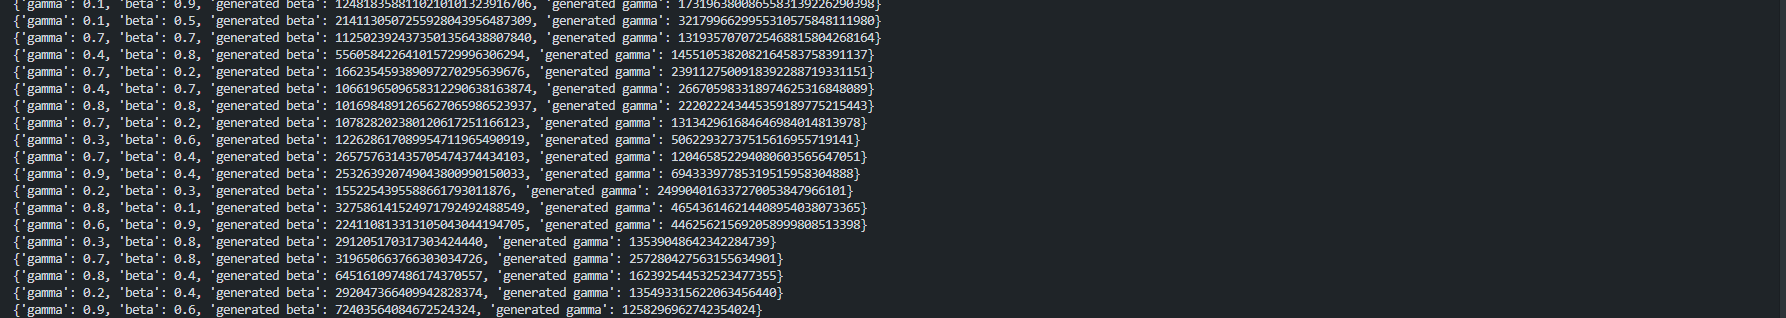
\includegraphics[width=0.6\textwidth]{images/3.png}
        \begin{center}
            fig.6
        \end{center} 

\end{center}

Como se aprecia hay una reduccion drástica de la longitud de dígitos devueltos en los parámetros gamma y beta, lo que sugiere que, con más computación se logren 
mejores cotas. Para este resultado para lograr este resutado se destinaron veinte minutos de computación, sin embargo los escasos resultados muestran la increible 
complejidad del modelo de regresión utilizado, sin embargo la predición de datos es considerablemente mas rápida, por lo tanto con este modelo tenemos buenos tiempo 
y resultado optimistas con respecto a la predicción, aunque el entrenamiento puede llegar a ser computacionalmente intenso a medida que le introduscamos mas datos de entrada.

\textbf{Modelo SI} \\

El modelo SI (Susceptible-Infectado) en este modelo, los individuos de la población se clasifican en dos categorías:
\begin{itemize}
    \item Susceptibles (S): Individuos que pueden contraer la enfermedad.
    \item  Infectados (I): Individuos que han contraído la enfermedad y pueden transmitirla.    
\end{itemize}

Supuestos del Modelo SI:La población es cerrada (no hay nacimientos, muertes ni migración), no hay recuperación ni inmunidad (los individuos infectados permanecen 
infectados para siempre), la enfermedad se transmite por contacto entre susceptibles e infectados. El modelo se describe mediante un sistema de ecuaciones diferenciales: \\

Tasa de cambio de los susceptibles (S): \\
   \[
   \frac{dS}{dt} = -\beta \cdot S \cdot I
   \]
   Donde:
   - \( \beta \) es la tasa de transmisión (probabilidad de contagio por contacto).
   - \( S \) es el número de susceptibles.
   - \( I \) es el número de infectados.

Tasa de cambio de los infectados (I):\\
   \[
   \frac{dI}{dt} = \beta \cdot S \cdot I
   \]

Población total (N): \\
   \[
   N = S + I
   \]
   La población total \( N \) se mantiene constante.

Número reproductivo básico (\( R_0 \)):
   \[
   R_0 = \beta \cdot N
   \]
   Si \( R_0 > 1 \), la enfermedad se propagará en la población. Todos los individuos eventualmente se infectarán (\( I \to N \) y \( S \to 0 \)). \\

   Las gráficas de datos usados para estimar el parámetro $\beta$ son las que siguen:



   \begin{center}
        
    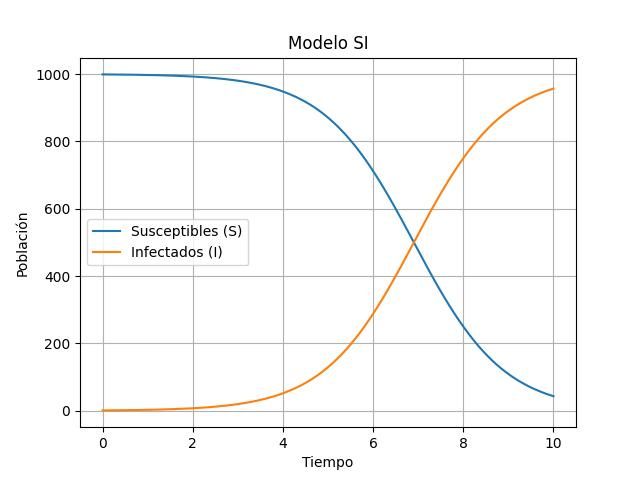
\includegraphics[width=0.6\textwidth]{images/plt02.jpg}
    \begin{center}
        fig.7
    \end{center} 
    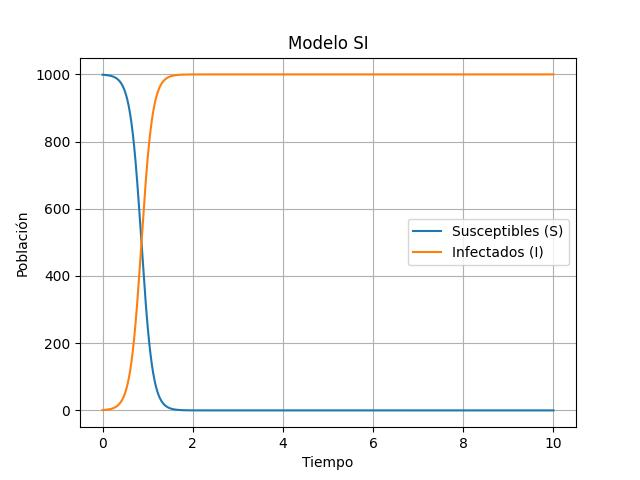
\includegraphics[width=0.6\textwidth]{images/plt12.jpg}
    \begin{center}
        fig.8
    \end{center} 
    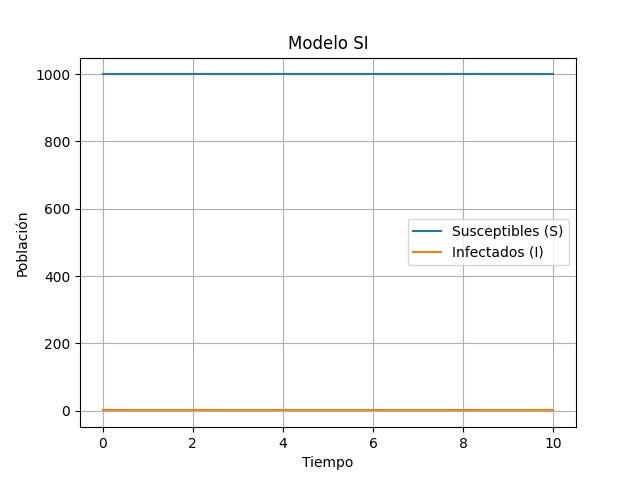
\includegraphics[width=0.6\textwidth]{images/plt22.jpg}
    \begin{center}
        fig.9
    \end{center} 
    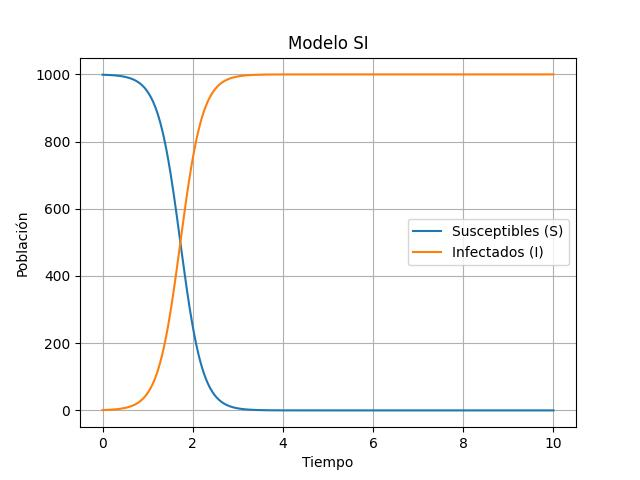
\includegraphics[width=0.6\textwidth]{images/plt32.jpg}
    

\end{center}

Al igual que con el modelo SIR los agentes han ido mejorando sus capacidades de predicción como se mostrara en la siguiente tabla, sin embargo el mínimo se consigue en 
$\beta=55015123$, siendo valor $\beta$ a aproximar igual a $0.009$. 

\begin{center}
     
 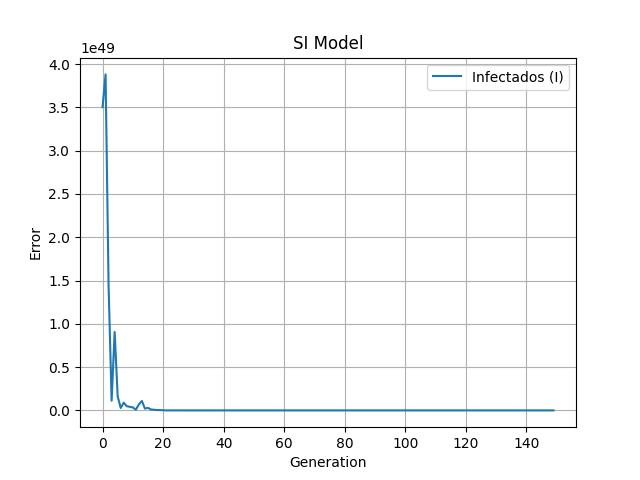
\includegraphics[width=0.6\textwidth]{images/plt1492.jpg} 
 \begin{center}
    
    fig.9
 \end{center}
\end{center}


Esta prueba al igual que la anterior nos demuestra que el modelo es capaz de mejorar con cada generación de datos que ocurre sin embargo el modelo usado 
para el agente coordinador no converge a minimos globales, por tanto nunca converge al grafo de conexiones entre agentes necesario para minimizar completamente la 
norma de la diferencia, además el costo computacional es significativo.